\makeatletter \def\NR@nopatch@beamer{} \makeatother %Temporary due to bug on 17 May

\documentclass{beamer}\usepackage[]{graphicx}\usepackage[]{xcolor}
% maxwidth is the original width if it is less than linewidth
% otherwise use linewidth (to make sure the graphics do not exceed the margin)
\makeatletter
\def\maxwidth{ %
  \ifdim\Gin@nat@width>\linewidth
    \linewidth
  \else
    \Gin@nat@width
  \fi
}
\makeatother

\definecolor{fgcolor}{rgb}{0.345, 0.345, 0.345}
\newcommand{\hlnum}[1]{\textcolor[rgb]{0.686,0.059,0.569}{#1}}%
\newcommand{\hlstr}[1]{\textcolor[rgb]{0.192,0.494,0.8}{#1}}%
\newcommand{\hlcom}[1]{\textcolor[rgb]{0.678,0.584,0.686}{\textit{#1}}}%
\newcommand{\hlopt}[1]{\textcolor[rgb]{0,0,0}{#1}}%
\newcommand{\hlstd}[1]{\textcolor[rgb]{0.345,0.345,0.345}{#1}}%
\newcommand{\hlkwa}[1]{\textcolor[rgb]{0.161,0.373,0.58}{\textbf{#1}}}%
\newcommand{\hlkwb}[1]{\textcolor[rgb]{0.69,0.353,0.396}{#1}}%
\newcommand{\hlkwc}[1]{\textcolor[rgb]{0.333,0.667,0.333}{#1}}%
\newcommand{\hlkwd}[1]{\textcolor[rgb]{0.737,0.353,0.396}{\textbf{#1}}}%
\let\hlipl\hlkwb

\usepackage{framed}
\makeatletter
\newenvironment{kframe}{%
 \def\at@end@of@kframe{}%
 \ifinner\ifhmode%
  \def\at@end@of@kframe{\end{minipage}}%
  \begin{minipage}{\columnwidth}%
 \fi\fi%
 \def\FrameCommand##1{\hskip\@totalleftmargin \hskip-\fboxsep
 \colorbox{shadecolor}{##1}\hskip-\fboxsep
     % There is no \\@totalrightmargin, so:
     \hskip-\linewidth \hskip-\@totalleftmargin \hskip\columnwidth}%
 \MakeFramed {\advance\hsize-\width
   \@totalleftmargin\z@ \linewidth\hsize
   \@setminipage}}%
 {\par\unskip\endMakeFramed%
 \at@end@of@kframe}
\makeatother

\definecolor{shadecolor}{rgb}{.97, .97, .97}
\definecolor{messagecolor}{rgb}{0, 0, 0}
\definecolor{warningcolor}{rgb}{1, 0, 1}
\definecolor{errorcolor}{rgb}{1, 0, 0}
\newenvironment{knitrout}{}{} % an empty environment to be redefined in TeX

\usepackage{alltt}
\usepackage{graphicx}
\usepackage{graphicx}
\usepackage{verbatim}
\usepackage{etoolbox}
\usepackage{everysel}
% \usepackage{enumitem}

%% This package allows text highlighting
\usepackage{soul}

%% This sets the theme of the presentation which controls
%% the formatting of the slides
\usetheme{Boadilla}

%% Turn off the navigation symbols
\setbeamertemplate{navigation symbols}{} 

%% Change the default itemize [ball]s to [circle]s
\setbeamertemplate{itemize items}[circle]

%% Change the default enumerate [ball]s to plain text
\setbeamertemplate{enumerate items}[default]

%% Load the enumitem package and ensure it works nicely with beamer
% \setitemize{label=\usebeamerfont*{itemize item}
%   \usebeamercolor[fg]{itemize item}
%   \usebeamertemplate{itemize item}}
% \setenumerate{label=\usebeamerfont*{enumerate item}
%   \usebeamercolor[fg]{enumerate item}
%   \usebeamertemplate{enumerate item}}

%% Set the author block so STATS 201/8 appears on every
\author{STATS 201/8}

%% Clear the date block
\date{}


\setbeamercolor{title}{bg=blue!40}
\setbeamerfont{title}{size=\LARGE,series=\bfseries}

%%Sectioning commands
\setbeamercolor{section title}{bg=blue!20}
\setbeamerfont{section title}{size=\large}

\setbeamertemplate{section page}{%
    \begingroup
        \begin{beamercolorbox}[sep=10pt,center,rounded=true,shadow=true]{section title}
        \usebeamerfont{section title}Section~\thechapter.\thesection \newline \insertsection\par
        \end{beamercolorbox}
		\vfill
    \endgroup
}

\newcommand{\BeginSection}[1]{\section{#1} \frame{\sectionpage}}
%\AtBeginSection[]{%
%    \begin{frame}
%        \sectionpage
%    \end{frame}
%}


%% This makes all equations blue
\AtBeginEnvironment{equation*}{\color{blue}}
\AtBeginEnvironment{align*}{\color{blue}}
\everymath{\color{blue}}

%% This puts a 0 point space between paragraphs, means we don't need to use vspace, or list environments if 
%% we don't want to
\setlength{\parskip}{0pt}


%% Russell: removes spaces after R input/output?
\setlength{\topsep}{0.5mm}

%% David: In addition to Russel's command to remove spaces after R input/output, these commands remove the space between R input/output.
%% Stackoverflow link: https://stackoverflow.com/questions/35734525/reduce-space-between-code-chunks-and-code-output-in-rmarkdown-beamer-presentatio
%% \setlength{\OuterFrameSep}{-2pt}
\makeatletter
\preto{\@verbatim}{\topsep=-1pt \partopsep=-1pt }
\makeatother

%% Some useful colors
\definecolor{darkgreen}{rgb}{0.176,0.486,0.031}
\definecolor{redbrown}{HTML}{950605}
\definecolor{darkred}{HTML}{d80605}


%% nice little macro for changing the font of R code
\newcommand{\rcode}[1]{\protect{\color{darkgreen}\texttt{#1}}}

%% macro for bold blue italics
\newcommand{\blueBoldEmph}[1]{{\color{blue}\textbf{\emph{#1}}}}

% ~iid macro
\newcommand{\iid }{\stackrel{iid}{\sim}}

%% Macro for t-test amd P-value
\newcommand{\ttest}{\emph{t}-test}
\newcommand{\pval}{\emph{P}-value}

%% Statistics operators 
\DeclareMathOperator{\Bias}{Bias}
\DeclareMathOperator{\Cov}{Cov}
\DeclareMathOperator*{\Cor}{Cor}
\DeclareMathOperator{\E}{E}
\DeclareMathOperator{\MSE}{MSE}
\DeclareMathOperator{\Odds}{Odds}
\DeclareMathOperator{\OR}{OR}
\DeclareMathOperator{\PMSE}{PMSE}
\DeclareMathOperator{\sd}{sd}
\DeclareMathOperator{\se}{se}
\DeclareMathOperator*{\Var}{Var}
\DeclareMathOperator{\logit}{logit}

%% Should see if can make this a mathop
\newcommand{\comb}[2]{\mbox{$\big(_{#2}^{#1}\big)$}}



\IfFileExists{upquote.sty}{\usepackage{upquote}}{}
\begin{document}
\newcommand{\thechapter}{12}




\title{Chapter \thechapter: \\ Linear models with two explanatory factor variables \\ (Two-way analysis of variance)}


\institute{University of Auckland}


\begin{frame}
\titlepage
\end{frame}



\begin{frame}[t]
\frametitle{Learning Outcomes}
In this chapter you will learn about:
\begin{center}
\vspace{16pt}
  \begin{itemize}
  \item Fitting a model with two explanatory factors, a.k.a., two-way ANOVA
  \item Interaction plots
  \item Interpretting the fitted model
  \item Pairwise comparisons using \rcode{emmeans}
  \item Simplifying the model where possible
  \item Relevant \rcode{R}-code
  \item Alternative parameterizations of the two-way ANOVA model\footnote{Optional section.}
  \end{itemize}
\end{center}
\end{frame}


% \begin{frame}
% \begin{center}
% {\huge Two explanatory factors}
% \end{center}
% \end{frame}



%%%%%%%%%%%%%%%%%%%%%%%%%%%%%%%%%%%%%%%%%%%%%%%%%%%%%%%%%%%%%%%%%%%%%%%%%%%%%%%%%%%%%%%%%%%
\BeginSection{Example: Using test success and attendance to explain exam score \\ ~ \\ Two-way ANOVA with interaction}
%%%%%%%%%%%%%%%%%%%%%%%%%%%%%%%%%%%%%%%%%%%%%%%%%%%%%%%%%%%%%%%%%%%%%%%%%%%%%%%%%%%%%%%%%%%


\begin{frame}[fragile]
\frametitle{Exam score vs test success and attendance}




In Chapter 8 we investigated whether the effect of a student's test mark on exam score changed depending on whether they regularly attend or not.
\smallskip

We saw that those who attended regularly ({\color{blue}blue} line and ``y'' for ``yes") got more `return' for each additional test mark than non-attenders.
\medskip

\begin{figure}
  \centering
  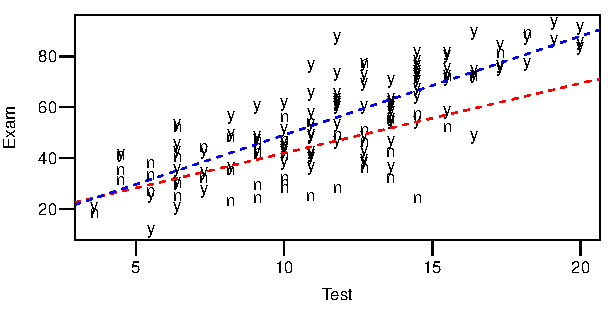
\includegraphics{figure/RC-H12-002}
\end{figure}

\end{frame}



\begin{frame}[fragile]
\frametitle{Exam score vs test success and attendance\ldots}

Here we will use the same two explanatory variables as in Chapter 8 but are going
to change the explanatory test score variable so that it only has two states
 --  passed or did not pass. \medskip

That is, we are going to use the dichotomous factor variable ``test success'',
rather than the raw numeric test score value. \medskip

We shall also be using attendance as a second explanatory factor.
\bigskip

For this example we shall use a two-way ANOVA, since there are two explanatory factors.
\medskip

First, read in the data and change the class of \rcode{Attend} to factor:
\medskip

\begin{knitrout}\scriptsize
\definecolor{shadecolor}{rgb}{0.969, 0.969, 0.969}\color{fgcolor}\begin{kframe}
\begin{alltt}
\hlstd{> }\hlcom{## Importing data into R}
\hlstd{> }\hlstd{Stats20x.df} \hlkwb{=} \hlkwd{read.table}\hlstd{(}\hlstr{"Data/STATS20x.txt"}\hlstd{,} \hlkwc{header}\hlstd{=T)}
\hlstd{> }\hlstd{Stats20x.df}\hlopt{$}\hlstd{Attend}\hlkwb{=}\hlkwd{factor}\hlstd{(Stats20x.df}\hlopt{$}\hlstd{Attend)}
\end{alltt}
\end{kframe}
\end{knitrout}
\end{frame}



\begin{frame}[fragile]
\frametitle{Exam score vs test success and attendance\ldots}

We next transform the numeric \rcode{Test} variable into a factor with two levels, \rcode{pass} and \rcode{nopass}.
\medskip

Let us create the new factor variable \rcode{Pass.test}:
\medskip

\begin{knitrout}\scriptsize
\definecolor{shadecolor}{rgb}{0.969, 0.969, 0.969}\color{fgcolor}\begin{kframe}
\begin{alltt}
\hlstd{> }\hlstd{Stats20x.df}\hlopt{$}\hlstd{Pass.test}\hlkwb{=}\hlkwd{with}\hlstd{(Stats20x.df,}
\hlstd{+ }                           \hlkwd{factor}\hlstd{(}\hlkwd{ifelse}\hlstd{(Test}\hlopt{>=}\hlnum{10}\hlstd{,}\hlstr{"pass"}\hlstd{,}\hlstr{"nopass"}\hlstd{)))}
\hlstd{> }\hlcom{## Check to see if the call above does what we expect}
\hlstd{> }\hlkwd{min}\hlstd{(Stats20x.df}\hlopt{$}\hlstd{Test[Stats20x.df}\hlopt{$}\hlstd{Pass.test}\hlopt{==}\hlstr{"pass"}\hlstd{])}
\end{alltt}
\begin{verbatim}
[1] 10
\end{verbatim}
\begin{alltt}
\hlstd{> }\hlkwd{max}\hlstd{(Stats20x.df}\hlopt{$}\hlstd{Test[Stats20x.df}\hlopt{$}\hlstd{Pass.test}\hlopt{==}\hlstr{"nopass"}\hlstd{])}
\end{alltt}
\begin{verbatim}
[1] 9.1
\end{verbatim}
\end{kframe}
\end{knitrout}
\bigskip

We can now examine whether passing the test results in better exam marks and vice-versa, on average. We can also ask the same question of regular attendance.

\medskip

\end{frame}



%%%%%%%%%%%%%%%%%%%%%%%%%%%%%%%%%%%%%%%%%%%%%%%%%%%%%%%%%%%%%%%%%%%%%%%%%%%%%%%%%%%%%%%%%%%
\BeginSection{Interaction plots }
%%%%%%%%%%%%%%%%%%%%%%%%%%%%%%%%%%%%%%%%%%%%%%%%%%%%%%%%%%%%%%%%%%%%%%%%%%%%%%%%%%%%%%%%%%%


\begin{frame}
\frametitle{Exam score vs test success and attendance\ldots}
\framesubtitle{\rcode{interactionPlots()}}

Let us see how these data explain \rcode{Exam} by using an \rcode{s20x} function \rcode{interactionPlots()}. 

\medskip

This is designed specifically for plotting a continuous $Y$ (in our case \rcode{Exam}) against two factor variables (here they are \rcode{Attend} and the newly created \rcode{Pass.test}).

\end{frame}


\begin{frame}[fragile]
\frametitle{Exam vs test success and attendance\ldots}
\framesubtitle{\rcode{interactionPlots()}\ldots}

\begin{knitrout}\scriptsize
\definecolor{shadecolor}{rgb}{0.969, 0.969, 0.969}\color{fgcolor}\begin{kframe}
\begin{alltt}
\hlstd{> }\hlkwd{interactionPlots}\hlstd{(Exam} \hlopt{~} \hlstd{Pass.test} \hlopt{+} \hlstd{Attend,} \hlkwc{data} \hlstd{= Stats20x.df)}
\end{alltt}
\end{kframe}
\end{knitrout}

\begin{knitrout}\scriptsize
\definecolor{shadecolor}{rgb}{0.969, 0.969, 0.969}\color{fgcolor}
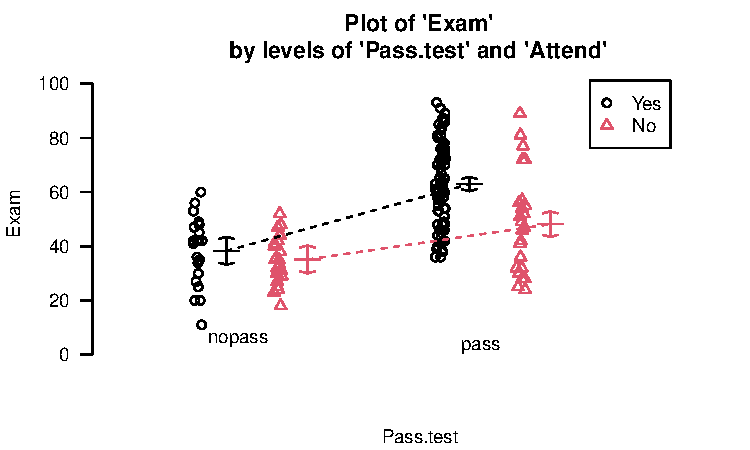
\includegraphics[width=\maxwidth]{figure/RC-H12-005-1} 
\end{knitrout}

\end{frame}



\begin{frame}[fragile]
\frametitle{Exam vs test success and attendance\ldots}

Here we see that `attenders' who pass the test seem to be doing markedly better than most other students. Note that we do not have parallel lines, thereby indicating that there could be an interaction between the two factors.
\medskip

In other words, the effect on exam score of passing the test may depend on whether a student regularly attended or not.
\bigskip \bigskip

As shown below, we can rearrange the layout of the interaction plot by reversing the order in which the explanatory variables are given in the right-hand side of the model formula argument.
\end{frame}


\begin{frame}[fragile]
\frametitle{Exam vs test success and attendance\ldots}
We still conclude the same insights as above. \medskip

\begin{knitrout}\scriptsize
\definecolor{shadecolor}{rgb}{0.969, 0.969, 0.969}\color{fgcolor}\begin{kframe}
\begin{alltt}
\hlstd{> }\hlkwd{interactionPlots}\hlstd{(Exam} \hlopt{~} \hlstd{Attend} \hlopt{+} \hlstd{Pass.test,} \hlkwc{data} \hlstd{= Stats20x.df)}
\end{alltt}
\end{kframe}
\end{knitrout}

\begin{knitrout}\scriptsize
\definecolor{shadecolor}{rgb}{0.969, 0.969, 0.969}\color{fgcolor}
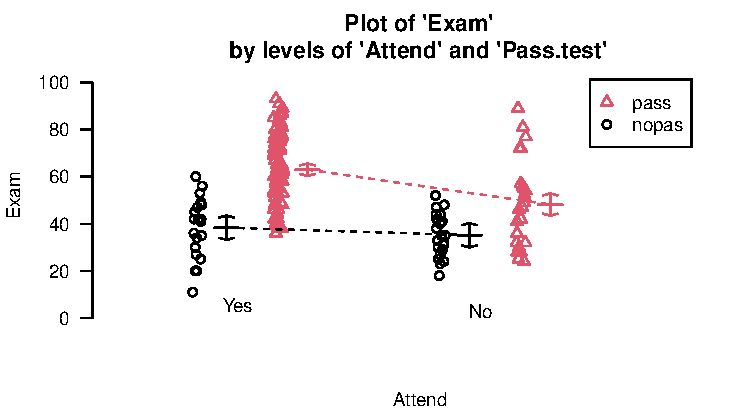
\includegraphics[width=\maxwidth]{figure/RC-H12-007-1} 
\end{knitrout}

\end{frame}



%%%%%%%%%%%%%%%%%%%%%%%%%%%%%%%%%%%%%%%%%%%%%%%%%%%%%%%%%%%%%%%%%%%%%%%%%%%%%%%%%%%%%%%%%%%
\BeginSection{Fitting the interaction model}
%%%%%%%%%%%%%%%%%%%%%%%%%%%%%%%%%%%%%%%%%%%%%%%%%%%%%%%%%%%%%%%%%%%%%%%%%%%%%%%%%%%%%%%%%%%


\begin{frame}[fragile]
\frametitle{Exam vs test success and attendance\ldots}
\framesubtitle{Assumption checks}
Let us fit the model with interaction, and check the assumptions.

\begin{knitrout}\scriptsize
\definecolor{shadecolor}{rgb}{0.969, 0.969, 0.969}\color{fgcolor}\begin{kframe}
\begin{alltt}
\hlstd{> }\hlstd{Exam.fit} \hlkwb{=} \hlkwd{lm}\hlstd{(Exam} \hlopt{~} \hlstd{Attend}\hlopt{*}\hlstd{Pass.test,} \hlkwc{data} \hlstd{= Stats20x.df)}
\hlstd{> }\hlkwd{plot}\hlstd{(Exam.fit,} \hlkwc{which}\hlstd{=}\hlnum{1}\hlstd{)}
\end{alltt}
\end{kframe}
\end{knitrout}



\begin{figure}
  \centering
  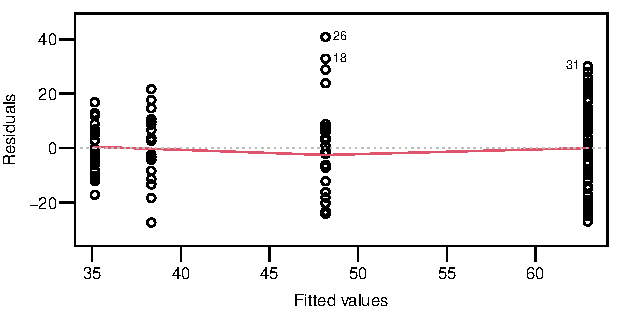
\includegraphics{figure/RC-H12-009}
\end{figure}

The \textbf{EOV} assumption seems to be okay.
\end{frame}


\begin{frame}[fragile]
\frametitle{Exam vs test success and attendance\ldots}
\framesubtitle{Assumption checks\ldots}
\begin{knitrout}\scriptsize
\definecolor{shadecolor}{rgb}{0.969, 0.969, 0.969}\color{fgcolor}\begin{kframe}
\begin{alltt}
\hlstd{> }\hlkwd{normcheck}\hlstd{(Exam.fit)}
\end{alltt}
\end{kframe}
\end{knitrout}



\begin{figure}
  \centering
  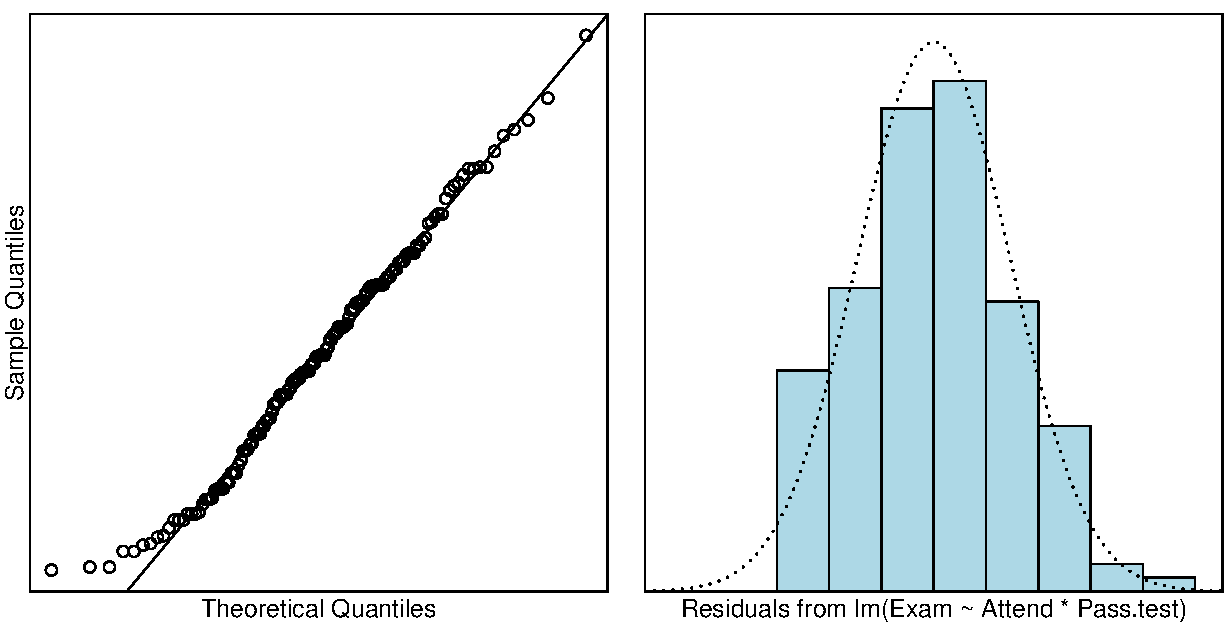
\includegraphics[scale = 0.5]{figure/RC-H12-011}
\end{figure}

The normality assumption seems to be reasonably good, other than a lack of large negative residuals.
\end{frame}


\begin{frame}
\frametitle{Exam vs test success and attendance\ldots}
\framesubtitle{Assumption checks\ldots}
\begin{knitrout}\scriptsize
\definecolor{shadecolor}{rgb}{0.969, 0.969, 0.969}\color{fgcolor}\begin{kframe}
\begin{alltt}
\hlstd{> }\hlkwd{cooks20x}\hlstd{(Exam.fit)}
\end{alltt}
\end{kframe}
\end{knitrout}



\begin{figure}
  \centering
  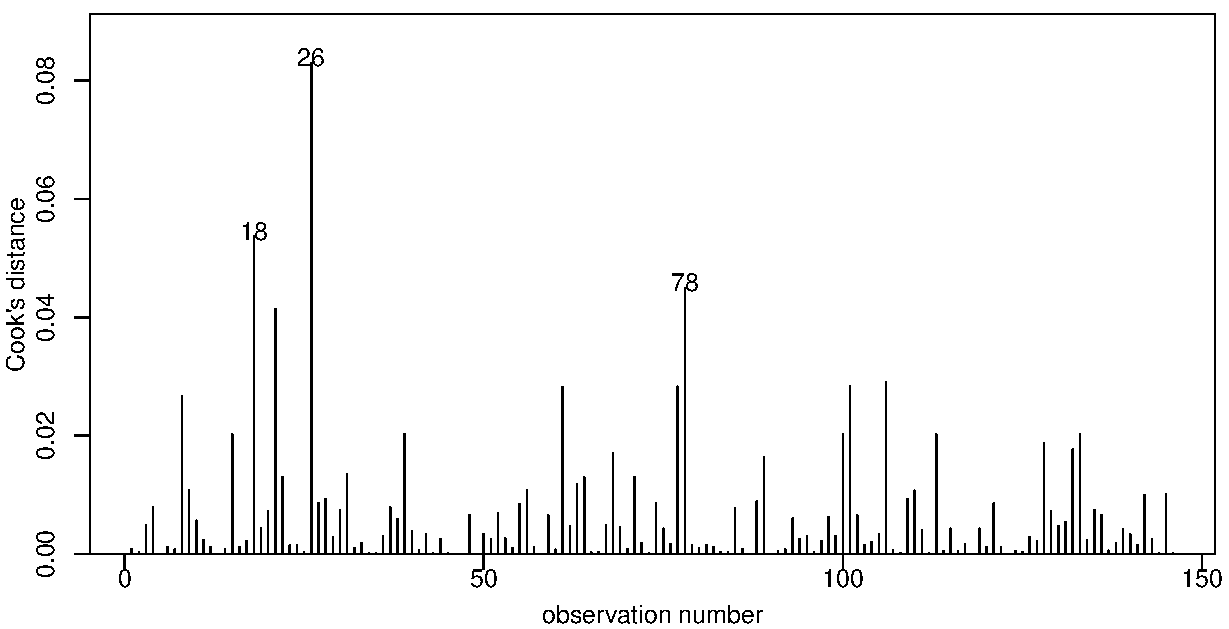
\includegraphics[scale = 0.5]{figure/RC-H12-013}
\end{figure}

No unduly influential data points.
\end{frame}


\begin{frame}[fragile]
\frametitle{Exam vs test success and attendance\ldots}
We conclude that we can trust the output. Let us see what it is telling us.

\begin{knitrout}\scriptsize
\definecolor{shadecolor}{rgb}{0.969, 0.969, 0.969}\color{fgcolor}\begin{kframe}
\begin{alltt}
\hlstd{> }\hlkwd{anova}\hlstd{(Exam.fit)}
\end{alltt}
\begin{verbatim}
Analysis of Variance Table

Response: Exam
                  Df  Sum Sq Mean Sq F value    Pr(>F)    
Attend             1  7630.8  7630.8  34.990 2.364e-08 ***
Pass.test          1 11076.9 11076.9  50.791 4.763e-11 ***
Attend:Pass.test   1   909.7   909.7   4.171   0.04297 *  
Residuals        142 30968.4   218.1                      
---
Signif. codes:  0 '***' 0.001 '**' 0.01 '*' 0.05 '.' 0.1 ' ' 1
\end{verbatim}
\end{kframe}
\end{knitrout}
\smallskip

The \pval{} of 0.043 is just under 0.05 and so establishes that there is a significant interaction: The effect of passing the test depends on whether the student has regularly attended lectures or not.
\smallskip

So, we cannot simply state the effect of passing the test, because the size of this effect depends on whether the student attended or not.
\smallskip

One way to think of this is that we have to consider all 4 (2 $\times$ 2) different test success/attendance possibilities separately.
\end{frame}


%anova output is Type 1 SS (sequential)
%anova(lm(Exam~Pass.test*Attend,data=Stats20x.df))

\begin{frame}[fragile, label={frame:two-way_refcellcoef}]
\frametitle{Exam vs test success and attendance\ldots}
Let us investigate what our model tells us in terms of the estimated parameters:

\begin{knitrout}\scriptsize
\definecolor{shadecolor}{rgb}{0.969, 0.969, 0.969}\color{fgcolor}\begin{kframe}
\begin{alltt}
\hlstd{> }\hlkwd{summary}\hlstd{(Exam.fit)}
\end{alltt}
\end{kframe}
\end{knitrout}

\begin{knitrout}\scriptsize
\definecolor{shadecolor}{rgb}{0.969, 0.969, 0.969}\color{fgcolor}\begin{kframe}
\begin{verbatim}
Coefficients:
                        Estimate Std. Error t value Pr(>|t|)    
(Intercept)               35.143      3.223  10.905  < 2e-16 ***
AttendYes                  3.190      4.557   0.700  0.48504    
Pass.testpass             13.017      4.371   2.978  0.00341 ** 
AttendYes:Pass.testpass   11.599      5.679   2.042  0.04297 *  
---
Residual standard error: 14.77 on 142 degrees of freedom
Multiple R-squared:  0.3878,	Adjusted R-squared:  0.3749 
F-statistic: 29.98 on 3 and 142 DF,  p-value: 4.452e-15
\end{verbatim}
\end{kframe}
\end{knitrout}

The \pval{} for interaction is the same as before.

\medskip

Note also that the $R^2=39\%$ can be obtained from the ANOVA table above as follows: $R^2 =100\times\left(1-\frac{30968}{30968+ 910 + 11077 + 7631} \right)$ is the proportion of variability that is explained by our model terms.
\end{frame}



\begin{frame}[fragile]
\frametitle{Exam vs test success and attendance\ldots}

The formula for the above two-way ANOVA can be written as:
\begin{align*}
\rcode{Exam} &= \beta_0 + \beta_1 \times \rcode{Attend}_{\rcode{Yes}} + \beta_2 \times \rcode{Pass.test}_{\rcode{pass}}\mbox{ } + \\ &\phantom{=}\mbox{ }\beta_3 \times \rcode{Attend}_{\rcode{Yes}} \times \rcode{Pass.test}_{\rcode{pass}} + \varepsilon 
\end{align*}
where $\rcode{Attend}_{\rcode{Yes}}$ and $\rcode{Pass.test}_{\rcode{pass}}$ are indicator variables, and $\varepsilon \iid N(0, \sigma^2)$.
\bigskip

This model is relative to the baseline levels of \rcode{Attend} and \rcode{Pass.test}.
These baselines are \rcode{No} and \rcode{nopass}, respectively, since they are the levels with the lowest alphanumeric value.
\end{frame}



\begin{frame}[fragile]
\frametitle{Exam vs test success and attendance\ldots}
\framesubtitle{Alternative parameterizations: the group means model}

As seen in the previous chapter, another option is to remove the baseline
with the addition of -1 in the model formula. 
One other complication is that we have to use \rcode{:} rather than \rcode{*} when specifying the interaction term.
\bigskip

\begin{knitrout}\scriptsize
\definecolor{shadecolor}{rgb}{0.969, 0.969, 0.969}\color{fgcolor}\begin{kframe}
\begin{alltt}
\hlstd{> }\hlstd{Exam.fitNoBaseline}\hlkwb{=}\hlkwd{lm}\hlstd{(Exam}\hlopt{~}\hlstd{Attend}\hlopt{:}\hlstd{Pass.test}\hlopt{-}\hlnum{1}\hlstd{,}\hlkwc{data}\hlstd{=Stats20x.df)}
\hlstd{> }\hlkwd{coef}\hlstd{(}\hlkwd{summary}\hlstd{(Exam.fitNoBaseline))}
\end{alltt}
\begin{verbatim}
                          Estimate Std. Error  t value     Pr(>|t|)
AttendNo:Pass.testnopass  35.14286   3.222594 10.90515 1.707299e-20
AttendYes:Pass.testnopass 38.33333   3.222594 11.89518 4.515124e-23
AttendNo:Pass.testpass    48.16000   2.953556 16.30577 2.405316e-34
AttendYes:Pass.testpass   62.94937   1.661505 37.88696 4.012344e-76
\end{verbatim}
\end{kframe}
\end{knitrout}

This is the group means model. It is simply giving the estimated group mean for each of the four combinations of attendance and test success.
\bigskip


\end{frame}



\begin{frame}[fragile]
\frametitle{Exam vs test success and attendance\ldots}
\framesubtitle{Alternative parameterizations: the means and effects model}

A further alternative is to use the means and effects model formula for the two-way ANOVA:
\[
\rcode{Exam}_{ijk} = \mu + \alpha_{i} + \beta_{j} + \gamma_{ij} + \epsilon_{ijk} \mbox{, where } \epsilon_{ijk} \iid N(0, \sigma^2)
\]
where: 
\begin{itemize}
  \item $\mu$ is the overall mean,
  \item $\alpha_i$s are the \rcode{Attend} effects relative to the overall mean,
  \item $\beta_j$s are the \rcode{Pass.test} effects relative to the overall mean,
  \item $\gamma_{ij}$s are the interaction effects between levels of \rcode{Attend} and \rcode{Pass.test} relative to the overall mean.
\end{itemize}

This is simply a different parameterization of the two-way ANOVA model. That is, there is no change to the model, but just in the way we choose to write it. 
\bigskip

In this course for Executive Summaries we will typically be interested in estimating relevant pairwise group differences, for which we will once again use \rcode{emmeans}.

\end{frame}



%%%%%%%%%%%%%%%%%%%%%%%%%%%%%%%%%%%%%%%%%%%%%%%%%%%%%%%%%%%%%%%%%%%%%%%%%%%%%%%%%%%%%%%%%%%
\BeginSection{Interpretting the output using pairwise differences}
%%%%%%%%%%%%%%%%%%%%%%%%%%%%%%%%%%%%%%%%%%%%%%%%%%%%%%%%%%%%%%%%%%%%%%%%%%%%%%%%%%%%%%%%%%%




\begin{frame}[fragile]
\frametitle{Exam vs test success and attendance}
\framesubtitle{Interpreting the output}

In studies in which {\em all} of the explanatory variables are factors, our interest typically lies in making statistical inferences about the sizes of pairwise differences between the means of different treatment combinations. 
\medskip

We could calculate these pairwise differences from the above output, but what we really need is Tukey-adjusted confidence intervals for the differences. These are needed because of the multi-comparisons problem. Once again, we will use the \rcode{emmeans()} function to perform these calculations for us.

\bigskip

In the field of statistics, pairwise comparisons are often called {\em contrasts}\footnote{ The term {\em contrasts} includes other more complicated forms of comparisons.} because they are comparing (i.e., contrasting) two different means. 

\end{frame}




\begin{frame}[fragile]
\frametitle{Exam vs test success and attendance}
\framesubtitle{Pairwise comparisons}

\begin{knitrout}\scriptsize
\definecolor{shadecolor}{rgb}{0.969, 0.969, 0.969}\color{fgcolor}\begin{kframe}
\begin{alltt}
\hlstd{> }\hlkwd{library}\hlstd{(emmeans)}
\hlstd{> }\hlstd{exam.pairs} \hlkwb{=} \hlkwd{pairs}\hlstd{(}\hlkwd{emmeans}\hlstd{(Exam.fit,} \hlopt{~} \hlstd{Attend}\hlopt{*}\hlstd{Pass.test),} \hlkwc{infer}\hlstd{=T)}
\hlstd{> }\hlstd{exam.pairs}
\end{alltt}
\begin{verbatim}
 contrast               estimate   SE  df lower.CL upper.CL t.ratio p.value
 No nopass - Yes nopass    -3.19 4.56 142    -15.0     8.66  -0.700  0.8969
 No nopass - No pass      -13.02 4.37 142    -24.4    -1.65  -2.978  0.0178
 No nopass - Yes pass     -27.81 3.63 142    -37.2   -18.38  -7.669  <.0001
 Yes nopass - No pass      -9.83 4.37 142    -21.2     1.54  -2.248  0.1155
 Yes nopass - Yes pass    -24.62 3.63 142    -34.0   -15.19  -6.789  <.0001
 No pass - Yes pass       -14.79 3.39 142    -23.6    -5.98  -4.364  0.0001

Confidence level used: 0.95 
Conf-level adjustment: tukey method for comparing a family of 4 estimates 
P value adjustment: tukey method for comparing a family of 4 estimates 
\end{verbatim}
\end{kframe}
\end{knitrout}
\bigskip

Typically (and in this course) we are only interested in within-level comparisons. 
That is, pairwise comparisons in which there is a level in common across the two treatment\footnote{The word {\em treatment} is often used to refer to a level of a factor variable.} combinations being compared.

\end{frame}



\begin{frame}[fragile, label={frame:refcell_intn_coeffs}]
\frametitle{Exam vs test success and attendance}
\framesubtitle{Pairwise comparisons\ldots}

To see only the within-level comparisons we can use the
\rcode{displayPairs} function from the \rcode{s20x} package.
\bigskip

\begin{knitrout}\scriptsize
\definecolor{shadecolor}{rgb}{0.969, 0.969, 0.969}\color{fgcolor}\begin{kframe}
\begin{alltt}
\hlstd{> }\hlkwd{displayPairs}\hlstd{(exam.pairs,} \hlkwd{c}\hlstd{(}\hlstr{"No"}\hlstd{,}\hlstr{"Yes"}\hlstd{),} \hlkwd{c}\hlstd{(}\hlstr{"nopass"}\hlstd{,}\hlstr{"pass"}\hlstd{))}
\end{alltt}
\end{kframe}
\end{knitrout}



\begin{knitrout}\scriptsize
\definecolor{shadecolor}{rgb}{0.969, 0.969, 0.969}\color{fgcolor}\begin{kframe}
\begin{verbatim}
 within               contrast        est       lwr        upr         pval
     No    No nopass - No pass -13.017143 -24.38137  -1.652912 1.776097e-02
    Yes  Yes nopass - Yes pass -24.616034 -34.04182 -15.190247 1.701486e-09
 nopass No nopass - Yes nopass  -3.190476 -15.03851   8.657554 8.969010e-01
   pass     No pass - Yes pass -14.789367 -23.59933  -5.979408 1.423139e-04
\end{verbatim}
\end{kframe}
\end{knitrout}

For example, the first row of the above output says that the estimated difference between the means of the two levels of \rcode{Pass.test} conditional on the level of \rcode{Attend} = \rcode{No} is \texttt{-13.02}. So, for students who do not regularly attend lectures, those who pass the test can expect to score 13 points higher in the exam than those who fail.
\end{frame}



\begin{frame}[fragile]
\frametitle{Exam vs test success and attendance\ldots}
\framesubtitle{Statements for the Executive Summary}



We interpret this output as follows (noting that the effect is always conditional on the level of the other factor):

\begin{itemize}
  \item We estimate that for students who attend regularly, those who pass the test can
expect to get 15 to 34 more marks in the exam than those who do not pass the test.

  \item For students who do not attend regularly, those who pass the test can expect to get
2 to 24 more marks in the exam than those who do not pass the test.

  \item For students who pass the test, those who regularly attend can expect to get between 6 and 24 more marks in the exam than those who do not attend regularly.

\item And, for those who do not pass the test, those who regularly attend can expect to get between 9 marks less and 15 more marks than those who do attend regularly.\footnote{Since this difference is not statistically significant, it should {\bf not} be reported in an Executive Summary.}
\end{itemize}
\end{frame}



\begin{frame}[fragile]
\frametitle{Exam vs test success and attendance\ldots}
\framesubtitle{Closing remarks}
Recall that the data used in this example are from a single STATS 20x summer school class. 
The above statements are only relevant to the population of students who could have taken the course that summer.
\bigskip \bigskip

Moreover, the data were collected pre-covid, so it is certainly the case that attendance at lectures would now not have anywhere near as much effect. 
\end{frame}



%%%%%%%%%%%%%%%%%%%%%%%%%%%%%%%%%%%%%%%%%%%%%%%%%%%%%%%%%%%%%%%%%%%%%%%%%%%%%%%%%%%%%%%%%%%
\BeginSection{Example 2: Using gender and attendance to explain exam score \\ ~ \\ Two-way ANOVA without interaction}
%%%%%%%%%%%%%%%%%%%%%%%%%%%%%%%%%%%%%%%%%%%%%%%%%%%%%%%%%%%%%%%%%%%%%%%%%%%%%%%%%%%%%%%%%%%

\begin{frame}[fragile]
\frametitle{Exam score vs gender and attendance}

Let us do another analysis where we will ask whether the effect of gender (on exam score) changes depending on whether the student attends regularly or not.

\end{frame}


\begin{frame}[fragile]
\frametitle{Exam vs gender and attendance}

\begin{knitrout}\scriptsize
\definecolor{shadecolor}{rgb}{0.969, 0.969, 0.969}\color{fgcolor}\begin{kframe}
\begin{alltt}
\hlstd{> }\hlkwd{interactionPlots}\hlstd{(Exam} \hlopt{~} \hlstd{Attend} \hlopt{+} \hlstd{Gender,} \hlkwc{data} \hlstd{= Stats20x.df)}
\end{alltt}
\end{kframe}
\end{knitrout}

\begin{knitrout}\scriptsize
\definecolor{shadecolor}{rgb}{0.969, 0.969, 0.969}\color{fgcolor}
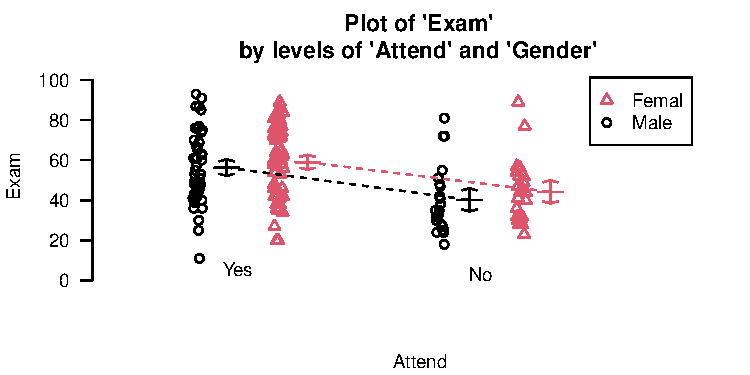
\includegraphics[width=\maxwidth]{figure/RC-H12-020-1} 
\end{knitrout}
Not so much going on here as our plots are parallel. Looks like there is an effect of attendance (no surprise), and the parallel lines suggests this effect is the same for both genders. There is little difference between genders.


\end{frame}


\begin{frame}[fragile]
\frametitle{Exam vs gender and attendance\ldots}
\framesubtitle{Assumption checks}

Let us fit an interaction model and check the assumptions.

\begin{knitrout}\scriptsize
\definecolor{shadecolor}{rgb}{0.969, 0.969, 0.969}\color{fgcolor}\begin{kframe}
\begin{alltt}
\hlstd{> }\hlstd{Exam.fit2} \hlkwb{=} \hlkwd{lm}\hlstd{(Exam} \hlopt{~} \hlstd{Attend}\hlopt{*}\hlstd{Gender,} \hlkwc{data} \hlstd{= Stats20x.df)}
\hlstd{> }\hlkwd{plot}\hlstd{(Exam.fit2,} \hlkwc{which}\hlstd{=}\hlnum{1}\hlstd{)}
\end{alltt}
\end{kframe}
\end{knitrout}



\begin{figure}
  \centering
  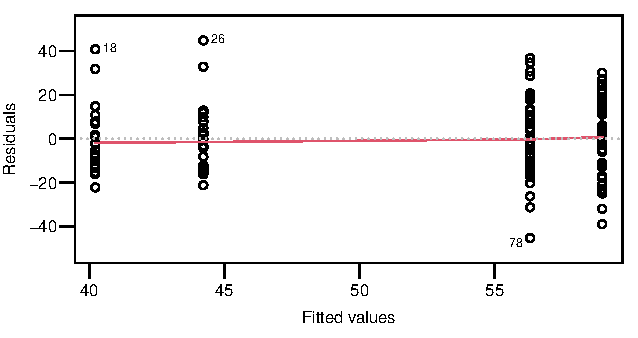
\includegraphics{figure/RC-H12-022}
\end{figure}

The EOV assumption seems to be okay.
\end{frame}


\begin{frame}[fragile]
\frametitle{Exam vs gender and attendance\ldots}
\framesubtitle{Assumption checks\ldots}

\begin{knitrout}\scriptsize
\definecolor{shadecolor}{rgb}{0.969, 0.969, 0.969}\color{fgcolor}\begin{kframe}
\begin{alltt}
\hlstd{> }\hlkwd{normcheck}\hlstd{(Exam.fit2)}
\end{alltt}
\end{kframe}
\end{knitrout}



\begin{figure}
  \centering
  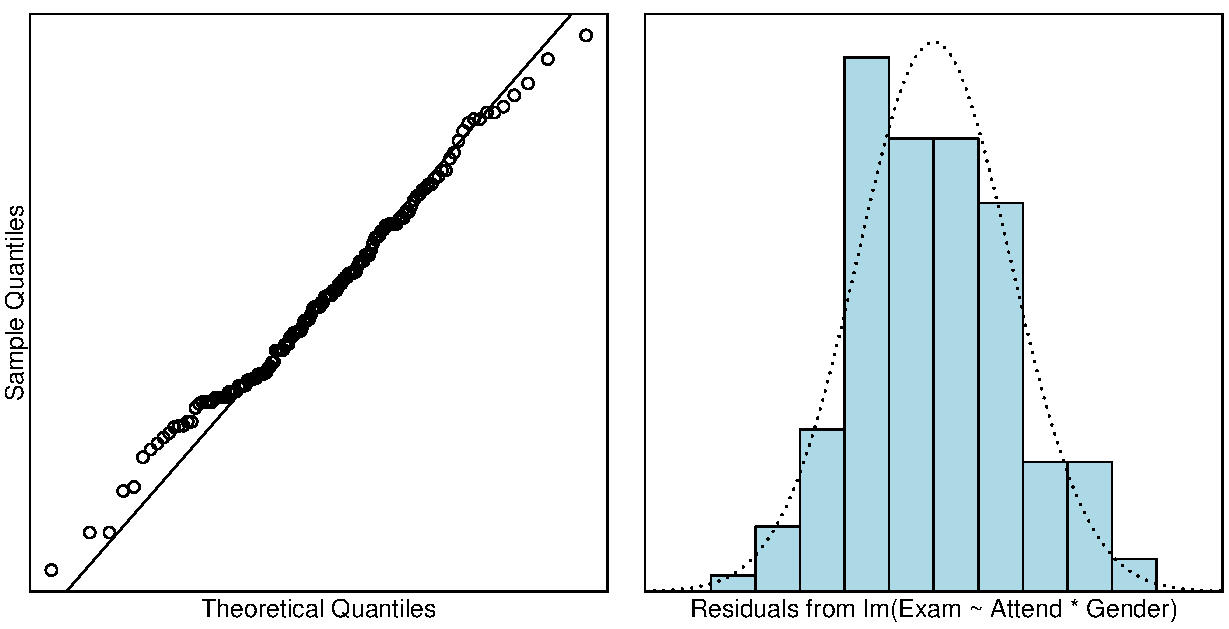
\includegraphics[scale = 0.5]{figure/RC-H12-024}
\end{figure}

The normality assumption seems to be okay.
\end{frame}


\begin{frame}[fragile]
\frametitle{Exam vs gender and attendance\ldots}
\framesubtitle{Assumption checks\ldots}

\begin{knitrout}\scriptsize
\definecolor{shadecolor}{rgb}{0.969, 0.969, 0.969}\color{fgcolor}\begin{kframe}
\begin{alltt}
\hlstd{> }\hlkwd{cooks20x}\hlstd{(Exam.fit2)}
\end{alltt}
\end{kframe}
\end{knitrout}



\begin{figure}
  \centering
  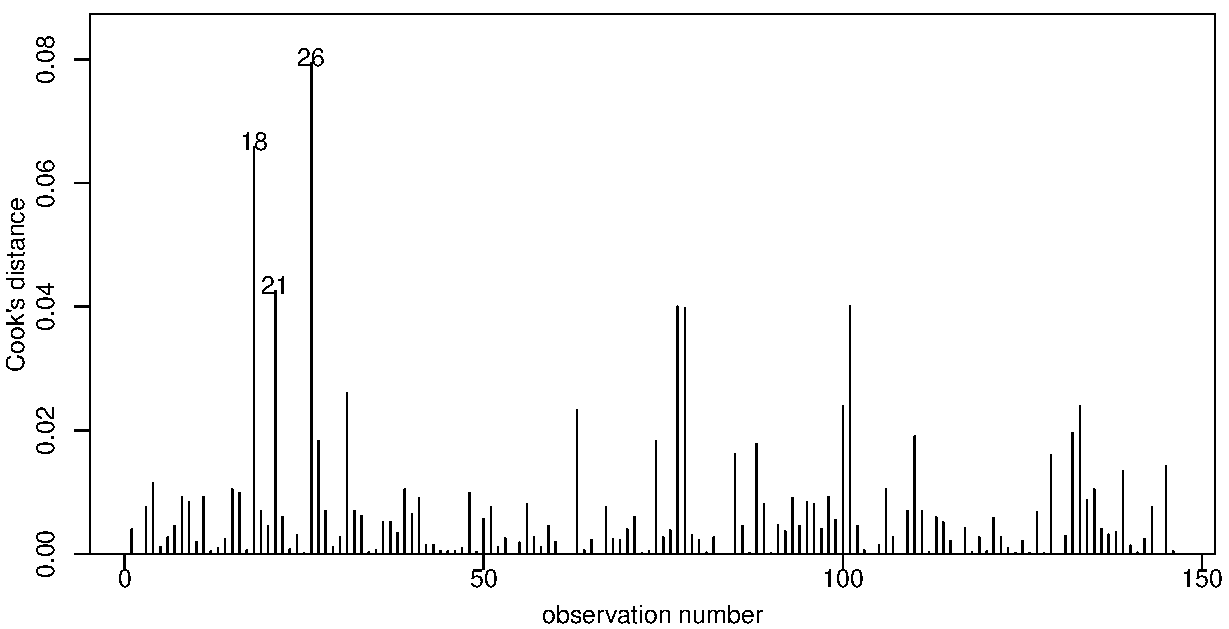
\includegraphics[scale = 0.5]{figure/RC-H12-026}
\end{figure}

No unduly influential data points.
\end{frame}



\begin{frame}[fragile]
\frametitle{Exam vs gender and attendance\ldots}
We can trust the model. Lets see what it is telling us.
\medskip

\begin{knitrout}\scriptsize
\definecolor{shadecolor}{rgb}{0.969, 0.969, 0.969}\color{fgcolor}\begin{kframe}
\begin{alltt}
\hlstd{> }\hlkwd{anova}\hlstd{(Exam.fit2)}
\end{alltt}
\begin{verbatim}
Analysis of Variance Table

Response: Exam
               Df Sum Sq Mean Sq F value    Pr(>F)    
Attend          1   7631  7630.8 25.4393 1.372e-06 ***
Gender          1    347   346.7  1.1557    0.2842    
Attend:Gender   1     14    13.9  0.0463    0.8300    
Residuals     142  42594   300.0                      
---
Signif. codes:  0 '***' 0.001 '**' 0.01 '*' 0.05 '.' 0.1 ' ' 1
\end{verbatim}
\end{kframe}
\end{knitrout}
\medskip

There is definitely no evidence of an interaction, so we'll apply Occam's razor\footnote{``With all things being equal, the simplest explanation tends to be the right one'', William of Ockham, 1287-1347.} and fit a simpler main-effects model (i.e., no interaction term).
\end{frame}



\begin{frame}[fragile]
\frametitle{Exam vs gender and attendance\ldots}
\framesubtitle{The main-effects model}
Recall that we use \rcode{+} rather that \rcode{*} in the model formula to fit the main-effects model.
\medskip

\begin{knitrout}\scriptsize
\definecolor{shadecolor}{rgb}{0.969, 0.969, 0.969}\color{fgcolor}\begin{kframe}
\begin{alltt}
\hlstd{> }\hlstd{Exam.fit3} \hlkwb{=} \hlkwd{lm}\hlstd{(Exam} \hlopt{~} \hlstd{Attend} \hlopt{+} \hlstd{Gender,} \hlkwc{data} \hlstd{= Stats20x.df)}
\hlstd{> }\hlkwd{anova}\hlstd{(Exam.fit3)}
\end{alltt}
\begin{verbatim}
Analysis of Variance Table

Response: Exam
           Df Sum Sq Mean Sq F value    Pr(>F)    
Attend      1   7631  7630.8 25.6101 1.264e-06 ***
Gender      1    347   346.7  1.1634    0.2826    
Residuals 143  42608   298.0                      
---
Signif. codes:  0 '***' 0.001 '**' 0.01 '*' 0.05 '.' 0.1 ' ' 1
\end{verbatim}
\end{kframe}
\end{knitrout}

We see that the gender is also not significant here\footnote{If it were significant then we could look at the output from \rcode{pairs(emmeans( Exam.fit3,$\sim$ Attend ), infer=T)} and \rcode{pairs(emmeans( Exam.fit3,$\sim$ Gender ), infer=T)} -- but this is pointless here since the factors only have two levels and there is only one pairwise comparison for each factor and so no multi-comparison issue.}, so we again apply Occam's razor and remove this term.
\end{frame}



\begin{frame}[fragile]
\frametitle{Exam vs gender and attendance\ldots}
Removal of the gender term reduces the model to one with just a factor with two levels. This is the two sample t-test scenario of Chapter 5. 

\medskip

\begin{knitrout}\scriptsize
\definecolor{shadecolor}{rgb}{0.969, 0.969, 0.969}\color{fgcolor}\begin{kframe}
\begin{alltt}
\hlstd{> }\hlstd{Exam.fit4} \hlkwb{=} \hlkwd{lm}\hlstd{(Exam} \hlopt{~} \hlstd{Attend,} \hlkwc{data} \hlstd{= Stats20x.df)}
\hlstd{> }\hlkwd{summary}\hlstd{(Exam.fit4)}
\end{alltt}
\end{kframe}
\end{knitrout}

\begin{knitrout}\scriptsize
\definecolor{shadecolor}{rgb}{0.969, 0.969, 0.969}\color{fgcolor}\begin{kframe}
\begin{verbatim}
Coefficients:
            Estimate Std. Error t value Pr(>|t|)    
(Intercept)   42.217      2.547  16.578  < 2e-16 ***
AttendYes     15.563      3.077   5.058 1.27e-06 ***
---
Residual standard error: 17.27 on 144 degrees of freedom
Multiple R-squared:  0.1508,	Adjusted R-squared:  0.145 
F-statistic: 25.58 on 1 and 144 DF,  p-value: 1.271e-06
\end{verbatim}
\end{kframe}
\end{knitrout}

\begin{knitrout}\scriptsize
\definecolor{shadecolor}{rgb}{0.969, 0.969, 0.969}\color{fgcolor}\begin{kframe}
\begin{alltt}
\hlstd{> }\hlkwd{confint}\hlstd{(Exam.fit4)}
\end{alltt}
\begin{verbatim}
                2.5 %   97.5 %
(Intercept) 37.184009 47.25077
AttendYes    9.480749 21.64447
\end{verbatim}
\end{kframe}
\end{knitrout}
\end{frame}


%%%%%%%%%%%%%%%%%%%%%%%%%%%%%%%%%%%%%%%%%%%%%%%%%%%%%%%%%%%%%%%%%%%%%%%%%%%%%%%%%%%%%%%%%%%
\BeginSection{Relevant \rcode{R}-code}
%%%%%%%%%%%%%%%%%%%%%%%%%%%%%%%%%%%%%%%%%%%%%%%%%%%%%%%%%%%%%%%%%%%%%%%%%%%%%%%%%%%%%%%%%%%




\begin{frame}[fragile]
\frametitle{Most of the \rcode{R}-code you need for this chapter}
You do not need to create indicator variables - \rcode{R} does that for you.
The baseline can be changed if you wish rather than having \rcode{R} choose it for you -- see relevant \rcode{R}-code from Chapter 9.  
\medskip

Use interaction-plots to inspect the data. Non-parallel lines indicate that interaction may exist.
\begin{knitrout}\scriptsize
\definecolor{shadecolor}{rgb}{0.969, 0.969, 0.969}\color{fgcolor}\begin{kframe}
\begin{alltt}
\hlstd{> }\hlkwd{interactionPlots}\hlstd{(Exam} \hlopt{~} \hlstd{Pass.test} \hlopt{+} \hlstd{Attend,} \hlkwc{data} \hlstd{= Stats20x.df)}
\end{alltt}
\end{kframe}
\end{knitrout}

Fit the interaction model  (use the \rcode{*} in the model formula)
\begin{knitrout}\scriptsize
\definecolor{shadecolor}{rgb}{0.969, 0.969, 0.969}\color{fgcolor}\begin{kframe}
\begin{alltt}
\hlstd{> }\hlstd{Exam.fit} \hlkwb{=} \hlkwd{lm}\hlstd{(Exam} \hlopt{~} \hlstd{Attend}\hlopt{*}\hlstd{Pass.test,} \hlkwc{data} \hlstd{= Stats20x.df)}
\end{alltt}
\end{kframe}
\end{knitrout}
and use the ANOVA table to see if there is evidence of interaction.

\begin{knitrout}\scriptsize
\definecolor{shadecolor}{rgb}{0.969, 0.969, 0.969}\color{fgcolor}\begin{kframe}
\begin{alltt}
\hlstd{> }\hlkwd{anova}\hlstd{(ExamTestAttend.fit)}
\end{alltt}
\end{kframe}
\end{knitrout}
In the first example we had evidence of interaction (small \pval{} associated with ``\rcode{:}'' part of the ANOVA output) and we inspect the pairwise interactions using \rcode{emmeans} to correct CIs for multi-comparisons:

\begin{knitrout}\scriptsize
\definecolor{shadecolor}{rgb}{0.969, 0.969, 0.969}\color{fgcolor}\begin{kframe}
\begin{alltt}
\hlstd{> }\hlstd{exam.pairs} \hlkwb{=} \hlkwd{pairs}\hlstd{(}\hlkwd{emmeans}\hlstd{(Exam.fit,} \hlopt{~} \hlstd{Attend}\hlopt{*}\hlstd{Pass.test),} \hlkwc{infer}\hlstd{=T)}
\hlstd{> }\hlkwd{displayPairs}\hlstd{(exam.pairs,} \hlkwd{c}\hlstd{(}\hlstr{"No"}\hlstd{,}\hlstr{"Yes"}\hlstd{),} \hlkwd{c}\hlstd{(}\hlstr{"nopass"}\hlstd{,}\hlstr{"pass"}\hlstd{))}
\end{alltt}
\end{kframe}
\end{knitrout}

\end{frame}



\begin{frame}[fragile]
\frametitle{Most of the \rcode{R}-code you need for this chapter}

If you don't have any evidence of interaction then simplify your model to a main-effects model and then see if the individual terms are significant. 
\medskip

The main-effects model replaces \rcode{*} with  a \rcode{+} in the model formula. E.g.,
\begin{knitrout}\scriptsize
\definecolor{shadecolor}{rgb}{0.969, 0.969, 0.969}\color{fgcolor}\begin{kframe}
\begin{alltt}
\hlstd{> }\hlstd{Exam.fit3}\hlkwb{=}\hlkwd{lm}\hlstd{(Exam} \hlopt{~} \hlstd{Attend}\hlopt{+}\hlstd{Gender,} \hlkwc{data} \hlstd{= Stats20x.df)}
\end{alltt}
\end{kframe}
\end{knitrout}
\bigskip

If both variables are significant in the main-effects model then use that model for inference (this model is referred to here as \rcode{additive.fit}) 

\begin{knitrout}\scriptsize
\definecolor{shadecolor}{rgb}{0.969, 0.969, 0.969}\color{fgcolor}\begin{kframe}
\begin{alltt}
\hlstd{> }\hlkwd{pairs}\hlstd{(}\hlkwd{emmeans}\hlstd{(additive.fit,} \hlopt{~} \hlstd{variable1),} \hlkwc{infer}\hlstd{=T)}
\end{alltt}
\end{kframe}
\end{knitrout}

\begin{knitrout}\scriptsize
\definecolor{shadecolor}{rgb}{0.969, 0.969, 0.969}\color{fgcolor}\begin{kframe}
\begin{alltt}
\hlstd{> }\hlkwd{pairs}\hlstd{(}\hlkwd{emmeans}\hlstd{(additive.fit,} \hlopt{~} \hlstd{variable2),} \hlkwc{infer}\hlstd{=T)}
\end{alltt}
\end{kframe}
\end{knitrout}
\bigskip

Otherwise, delete non-significant variables until you have the simplest model possible.
\end{frame}



%%%%%%%%%%%%%%%%%%%%%%%%%%%%%%%%%%%%%%%%%%%%%%%%%%%%%%%%%%%%%%%%%%%%%%%%%%%%%%%%%%%%%%%%%%%
\BeginSection{Alternative parameterizations of the two-way ANOVA model \\ ~ \\
(This is an optional Section \\ - your lecturer will advise if it is examinable)}
%%%%%%%%%%%%%%%%%%%%%%%%%%%%%%%%%%%%%%%%%%%%%%%%%%%%%%%%%%%%%%%%%%%%%%%%%%%%%%%%%%%%%%%%%%%


\begin{frame}[fragile, label={frame:2way_RefCellModel}]
\frametitle{Alternative parameterizations of two-way ANOVA}
\framesubtitle{The reference cell model}
  
Recall the reference cell model we used to represent \rcode{Exam} score:
  
\vspace{-5mm}

\begin{align*}
\rcode{Exam} &= \beta_0 + \beta_1 \times \rcode{Attend}_{\rcode{Yes}} + \beta_2 \times \rcode{Pass.test}_{\rcode{pass}}\mbox{ } + \\ &\phantom{=}\mbox{ }\beta_3 \times \rcode{Attend}_{\rcode{Yes}} \times \rcode{Pass.test}_{\rcode{pass}} + \varepsilon,
\end{align*}

\vspace{-5mm}

where $\varepsilon \iid N(0, \sigma^2)$.

\medskip

The parameter $\beta_0$ denotes the overall true baseline mean exam score. Notice that neither the \rcode{no} level of \rcode{Attend} nor the \rcode{nopass} level of \rcode{Pass.test} appear as subscripts in the above model. This tells us that these are the baseline levels, i.e. $\beta_0$ denotes the mean over \rcode{Exam} scores from students who neither regularly attended lectures nor passed the test.

\medskip

So, what do the parameters $\beta_1,\beta_2,\text{ and }\beta_3$ represent? To help us answer this question we consider the means model\footnote{We first encountered the means model for the single factor male fruitflies study in Chapter 11.} formulation for \rcode{Exam} score. 
  
\end{frame}  


\begin{frame}[fragile]
\frametitle{Alternative parameterizations of two-way ANOVA}
\framesubtitle{The means model}

The means model parameterization for exam score is

\vspace{-5mm}

\begin{align*}
\rcode{Exam}_{ijk} &= \mu_{ij} + \varepsilon_{ijk},
\end{align*}

\vspace{-5mm}

where $\mu_{ij}$ denotes the true mean exam score of 20x students who are in the $i$th level of \rcode{Attend} and $j$th level of \rcode{Pass.test} ($i=\rcode{no}$ or $\rcode{yes}$; $j=\rcode{nopass}$ or $\rcode{pass}$). The error term $\varepsilon_{ijk} \iid N(0, \sigma^2)$ denotes the deviation of the $k$th student's exam score from the mean exam score, $\mu_{ij}$.

\bigskip

But, how can we use $\mu_{ij}$ to assess whether one or both of \rcode{Attend} and \rcode{Pass.test} have an effect on \rcode{Exam} score? 

\end{frame}


\begin{frame}[fragile]
\frametitle{Alternative parameterizations of two-way ANOVA}
\framesubtitle{Relating the means and reference cell models}

\medskip

We decompose each mean response, $\mu_{ij}$, into four terms:

\medskip

\begin{enumerate}
\setlength\itemsep{0.55em}
  \item $\mu_{11}$, the baseline or reference-level mean response;
  \item $\mu_{i1}-\mu_{11}$, the {\em main effect}\footnote{A main effect is defined as the difference between the mean response when all factors, except the one of interest, are at the baseline level and the reference-level mean.} of the $i$th level of the first factor, where $i$ does not equal the baseline level;
  \item $\mu_{1j}-\mu_{11}$, the {\em main effect} of the $j$th level of the second factor, where $j$ does not equal the baseline level;
  \item $\text{Interaction}$, the part of $\mu_{ij}$ that is left over after eliminating the contributing components defined by terms 1--3 above, i.e.
  \begin{align*}
    \text{Interaction} &= \mu_{ij} - \mu_{11} - (\mu_{i1}-\mu_{11}) - (\mu_{1j}-\mu_{11}) \\
                       &= \mu_{ij} - \mu_{i1} - \mu_{1j} + \mu_{11}
  \end{align*}
  
\end{enumerate}

\end{frame}


\begin{frame}[fragile]
\frametitle{Alternative parameterizations of two-way ANOVA}
\framesubtitle{Relating the means and reference cell models}

We now have the tools to re-express the mean \rcode{Exam} score in terms of the main effects of the $i$th level of \rcode{Attend} and the $j$th level of \rcode{Pass.test}, and their interaction, i.e.

\vspace{-7.5mm}

\begin{align*}
   \mu_{ij} &= \mu_{11} + (\mu_{1j}-\mu_{11}) + (\mu_{i1}-\mu_{11})%\\
            %&\phantom{=}
            +(\mu_{ij} - \mu_{i1} - \mu_{1j} + \mu_{11}).
\end{align*}

\vspace{-6mm}

The following two-way table\footnote{\scriptsize More generally, differences in the first row of a two-way reference model decomposition table correspond to the main effects of the column factor. The differences in the first column correspond to the row factor main effects. The terms in each of the of the remaining cells, except the reference cell, correspond to interaction effects.} illustrates how each term in the above decomposition relates to each combination of the levels of \rcode{Attend} and \rcode{Pass.test}:

\bigskip

\begin{center}
  \footnotesize
  \renewcommand{\arraystretch}{1.15}
  \begin{tabular}{|c|c|c|}
    \hline
           &\multicolumn{2}{c|}{Pass.test}\\  
    \cline{2-3}           
    Attend & \rcode{nopass} & \rcode{pass}\\
     \hline
    \rcode{no}  & $\mu_{11}$     & $\mu_{i1}-\mu_{11}$  \\ \hline
    \rcode{yes} & $ \mu_{1j} - \mu_{11}$ & $ \mu_{ij} - \mu_{11} - (\mu_{i1}-\mu_{11}) - (\mu_{1j}-\mu_{11})$ \\ \hline
  \end{tabular}
\end{center}

\medskip

% \medskip
% 
% To enable each of the parameters in the above table to have a uniquely determined value, we must set some constraints.\footnote{The details of why and how are beyond the scope of this course.}  

\end{frame}


\begin{frame}[fragile]
\frametitle{Alternative parameterizations of two-way ANOVA}
\framesubtitle{Relating the means and reference cell models}

\begin{center}
\footnotesize
\renewcommand{\arraystretch}{1.15}
{\setlength{\tabcolsep}{2.2pt} 
\begin{tabular}{cccccclr}
      \hline
      \multicolumn{2}{c}{Factors}&& \multicolumn{5}{c}{Parameterization} \\
      \cline{1-2}\cline{4-8}
      \rcode{Attend} & \rcode{Pass.test} && Means & Estimate\footnote{See estimates of \rcode{Attend}$\times$\rcode{Pass.test} treatment means on slide~\ref{frame:emmeans}.} &&
         Reference cell & Estimate\footnote{See regression coefficients table on slide~\ref{frame:two-way_refcellcoef}.} \\
      \hline
      \rcode{no}  & \rcode{nopass} && $\mu_{11}$ & 35.1 && $\beta_0 = \mu_{11}$ & 35.1 \\
      \rcode{yes} & \rcode{nopass} && $\mu_{21}$ & 38.3 && $\beta_1 = \mu_{21} - \mu_{11}$ & $3.2$  \\
      \rcode{no}  & \rcode{pass}   && $\mu_{12}$ & 48.2 && $\beta_2 = \mu_{12} - \mu_{11}$ & $13.1$ \\
      \rcode{yes} & \rcode{pass}   && $\mu_{22}$ & 62.9 && $\beta_3 = \mu_{22} - \mu_{21} - \mu_{12} + \mu_{11}$ & $11.5$ \\
      \hline
   \end{tabular}}
\end{center}

\bigskip

From the above table we see that:
\begin{itemize}
  \item $\beta_1$ represents the effect of \rcode{Attend = yes} at the reference level of \rcode{Pass.test = nopass}
  \item $\beta_2$ represents the effect of \rcode{Pass.test = pass} at the reference level of \rcode{Attend = no}
  \item $\beta_3$ represents the \rcode{Attend} $x$ \rcode{Pass.test} interaction effect when \rcode{Attend = yes} and \rcode{Pass.test = pass}
\end{itemize}

\end{frame}


\begin{frame}[fragile]
\frametitle{Alternative parameterizations of two-way ANOVA}
\framesubtitle{The reference cell model}

The values in the \rcode{Estimate} column of the regression summary table\footnote{See slide~\ref{frame:two-way_refcellcoef}; Coefficients rounded to 2 decimal places.} result in the following equation for predicted longevity:
    

    
\medskip
  
\begin{align*}
  \widehat{\rcode{Exam}} &=35.14+3.19\times \rcode{Attend}_{\rcode{Yes}} + 13.02\times \rcode{Pass.test}_{\rcode{pass}} \\
  &\phantom{=}+ 11.60\times \rcode{Attend}_{\rcode{Yes}} \times \rcode{Pass.test}_{\rcode{pass}}
\end{align*}
  
\end{frame}
  


\begin{frame}[fragile]
\frametitle{Alternative parameterizations of two-way ANOVA}
\framesubtitle{Relating the means and effects models}

\medskip

We saw in Chapter 11 that the effects model offers an alternative to the reference model parameterization.\footnote{\scriptsize The effects model is the default parameterization used in the analysis of data from designed experiments and, therefore, in STATS 240 (Design and Structured Data).} To relate the means and effects models we use an alternative decomposition of each mean response, $\mu_{ij}$, into:

\medskip

\begin{enumerate}
\setlength\itemsep{0.55em}
  \item $\mu=\mu_{\cdot\cdot}$, the reference overall mean response;
  \item $\alpha_i = \mu_{i\cdot}-\mu$, the {\em main effect} of the $i$th level of the first factor\footnote{\scriptsize The distance between the mean response of the first (second) factor at the $i$th ($j$th) level and the overall mean.\label{fn:maineffect}};
  \item $\pi_j = \mu_{\cdot j}-\mu$, the {\em main effect} of the $j$th level of the second factor\footnotemark[\getrefnumber{fn:maineffect}];
  \item $(\alpha\tau)_{ij}$, the interaction effect reflecting the component of $\mu_{ij}$ left over after eliminating the components corresponding to the terms defined in 1--3 above, i.e. $(\alpha\tau)_{ij} = \mu_{ij} - \mu - \alpha_i - \pi_j$.
  
\end{enumerate}

\end{frame}


\begin{frame}[fragile]
\frametitle{Alternative parameterizations of two-way ANOVA}
\framesubtitle{The effects model}

It directly follows from point 4 above that we can re-express the mean \rcode{Exam} score, $\mu_{ij}$, in terms of $\alpha_i$, the  effect of the $i$th level of \rcode{Attend}, $\pi_j$, the effect of the $j$th level of \rcode{Pass.test}, and their interaction, $(\alpha\pi)_{ij}$, i.e.

\vspace{-5.5mm}

\begin{align*}
   \mu_{ij} &= \mu + \alpha_i + \pi_j + (\alpha\pi)_{ij}.
\end{align*}

\vspace{-5.5mm}

This means that the effects model formula for the two-way ANOVA is
\[
\rcode{Exam}_{ijk} = \mu + \alpha_{i} + \pi_{j} + (\alpha\pi)_{ij} + \epsilon_{ijk},
\]

where $\epsilon_{ijk} \iid N(0, \sigma^2)$.

\end{frame}


\begin{frame}[fragile]
\frametitle{Alternative parameterizations of two-way ANOVA}
\framesubtitle{Relating the means and effects models}

The following two-way layout illustrates how the above decomposition of $\mu_{ij}$ relates to each combination of the levels of \rcode{Attend} and \rcode{Pass.test}:

\medskip

\begin{center}
  \footnotesize
  \renewcommand{\arraystretch}{1.15}
  \begin{tabular}{|c|c|c|c|c|}
    \hline
           &\multicolumn{2}{c|}{Pass.test} & & \\
    \cline{2-3}
    Attend & \rcode{nopass} & \rcode{pass} & Row mean & $\alpha_i$, Row effect \\
     \hline
    \rcode{no}  & $\mu_{11}=35.1$ & $\mu_{12}=48.2$ & $\mu_{1\cdot}=41.7$ &  \\ \hline
    \rcode{yes} & $\mu_{21}=38.3$ & $\mu_{22}=62.9$ & $\mu_{2 \cdot}=50.6$ & \\ \hline
    Column mean & $\mu_{\cdot 1}=36.7$ & $\mu_{\cdot 2}=55.6$ & $\mu=52.9$ & \\ \hline
    $\pi_i$, Column effect &  &  & &  \\ \hline
  \end{tabular}
\end{center}

\medskip

\begin{knitrout}\scriptsize
\definecolor{shadecolor}{rgb}{0.969, 0.969, 0.969}\color{fgcolor}\begin{kframe}
\begin{alltt}
\hlstd{> }\hlkwd{emmeans}\hlstd{(Exam.fit,}\hlopt{~}\hlstd{Attend)}
\end{alltt}
\begin{verbatim}
 Attend emmean   SE  df lower.CL upper.CL
 No       41.7 2.19 142     37.3     46.0
 Yes      50.6 1.81 142     47.1     54.2

Results are averaged over the levels of: Pass.test 
Confidence level used: 0.95 
\end{verbatim}
\begin{alltt}
\hlstd{> }\hlkwd{emmeans}\hlstd{(Exam.fit,}\hlopt{~}\hlstd{Pass.test)}
\end{alltt}
\begin{verbatim}
 Pass.test emmean   SE  df lower.CL upper.CL
 nopass      36.7 2.28 142     32.2     41.2
 pass        55.6 1.69 142     52.2     58.9

Results are averaged over the levels of: Attend 
Confidence level used: 0.95 
\end{verbatim}
\end{kframe}
\end{knitrout}

% \begin{center}
%   \footnotesize
%   \renewcommand{\arraystretch}{1.15}
%   \begin{tabular}{|c|c|c|c|}
%     \hline
%            &\multicolumn{2}{c|}{Pass.test} & \\
%     \cline{2-3}
%     Attend & \rcode{nopass} & \rcode{pass} & Row effect \\ \hline
%      \rcode{no}    & $(\alpha\pi)_{11}$        & $(\alpha\pi)_{12}$         & $\alpha_1=\mu_{1\cdot}-\mu$ \\ \hline
%      \rcode{yes}   & $(\alpha\pi)_{21}$        & $(\alpha\pi)_{22}$         & $\alpha_2=\mu_{2\cdot}-\mu$ \\ \hline
%      Column effect & $\pi_1=\mu_{\cdot 1}-\mu$ & $\pi_2=\mu_{\cdot 2}-\mu$  &  \\ \hline
%   \end{tabular}
% \end{center}

\end{frame}
%\end{document}


% \begin{frame}[fragile]
% \frametitle{Alternative parameterizations of the two-factor linear model}
% \framesubtitle{Relating the means and reference cell models}
% 
% For the reference cell model\footnote{Recall from slide~\ref{frame:2way_RefCellModel} that $\beta_0$ represents the mean response when each factor is at its designated reference level.} we set (constrain) $\mu=\beta_0$ and $\alpha_1 = \pi_1 = 0$.  This means that for the 20x exam score study 
% 
% $$ \mu = \beta_0 = \mu_{\rcode{no},\rcode{nopass}} \qquad \text{and} \qquad \alpha_\rcode{no} = \pi_\rcode{nopass} = 0.$$
% 
% \medskip
% 
% \end{frame}




% \begin{frame}[fragile]
% \frametitle{Alternative parameterizations of the linear model}
% \framesubtitle{The reference cell model}
% 
% For the reference cell model we set $\mu$ to represent the mean response when each factor is at its designated reference level and $\alpha_1 = \pi_1 = 0$. It follows, therefore, that for the exam score study $\mu = \mu_{\rcode{no}, \rcode{nopass}}$ and $\alpha_\rcode{no} = \pi_\rcode{nopass} = 0$.
% 
% \medskip
% 
% \begin{center}
%   \footnotesize
%   \renewcommand{\arraystretch}{1.15}
%   \begin{tabular}{|c|c|c|c|}
%     \hline
%            &\multicolumn{2}{c|}{Pass.test} & \multicolumn{1}{c|}{}\\  
%     \cline{2-3}           
%     Attend & \rcode{nopass} & \rcode{pass} & Col 2 $-$ Col 1\\
%      \hline
%     \rcode{no}  & $\beta_0=\mu_{\rcode{no},\rcode{nopass}}$  & $\mu_{\rcode{no},\rcode{pass}}$ & $\beta_1$ \\ \hline
%     \rcode{yes} & $\mu_{\rcode{yes},\rcode{nopass}}$         & $\mu_{\rcode{yes},\rcode{pass}}$ & $-$ \\ \hline
%     Row 2 $-$ Row 1 & $\beta_2$ & $-$ & $-$ \\ \hline
%   \end{tabular}
% \end{center}
% 
% \bigskip
% 
% From the above table we see that:
% \begin{itemize}
%   %\item $\beta_1 = \mu_{\rcode{no},\rcode{pass}}-\mu_{\rcode{no},\rcode{nopass}} =\mu_{\rcode{no},\rcode{pass}}-\beta_0,$
%   \item $\beta_1 = \mu_{\rcode{no},\rcode{pass}}-\beta_0$, i.e. the effect of \rcode{Pass.test} conditional on \rcode{Attend = no}
%   %\item $\beta_2 = \mu_{\rcode{no},\rcode{pass}}-\mu_{\rcode{no},\rcode{nopass}} = \mu_{\rcode{yes},\rcode{nopass}}-\beta_0,$
%   \item $\beta_2 = \mu_{\rcode{yes},\rcode{nopass}}-\beta_0$, i.e. the effect of \rcode{Attend} conditional on \rcode{Pass.test = nopass}
%   \item $\beta_3=$?
% \end{itemize}
% 
% \end{frame}


\begin{frame}[fragile]
\frametitle{Alternative parameterizations of two-way ANOVA}
\framesubtitle{Relating the means and effects models}

\begin{center}
\footnotesize
\renewcommand{\arraystretch}{1.15}
{\setlength{\tabcolsep}{2.2pt} 
\begin{tabular}{cccccclr}
      \hline
      \multicolumn{2}{c}{Factors}&& \multicolumn{5}{c}{Parameterization} \\
      \cline{1-2}\cline{4-8}
      \rcode{Attend} & \rcode{Pass.test} && Means & Estimate\footnote{See estimates of \rcode{Attend}$\times$\rcode{Pass.test} treatment means on slide~\ref{frame:emmeans}.} &&
         Reference cell & Estimate\footnote{See regression coefficients table on slide~\ref{frame:two-way_refcellcoef}.} \\
      \hline
      \rcode{no}  & \rcode{nopass} && $\mu_{11}$ & 35.1 && $\beta_0 = \mu_{11}$ & 35.1 \\
      \rcode{yes} & \rcode{nopass} && $\mu_{21}$ & 38.3 && $\beta_1 = \mu_{21} - \mu_{11}$ & $3.2$  \\
      \rcode{no}  & \rcode{pass}   && $\mu_{12}$ & 48.2 && $\beta_2 = \mu_{12} - \mu_{11}$ & $13.1$ \\
      \rcode{yes} & \rcode{pass}   && $\mu_{22}$ & 62.9 && $\beta_3 = \mu_{22} - \mu_{21} - \mu_{12} + \mu_{11}$ & $11.5$ \\
      \hline
   \end{tabular}}
\end{center}

\bigskip

From the above table we see that:
\begin{itemize}
  \item $\beta_1$ represents the effect of \rcode{Attend = yes} at the reference level of \rcode{Pass.test = nopass}
  \item $\beta_2$ represents the effect of \rcode{Pass.test = pass} at the reference level of \rcode{Attend = no}
  \item $\beta_3$ represents the \rcode{Attend} $x$ \rcode{Pass.test} interaction effect when \rcode{Attend = yes} and \rcode{Pass.test = pass}
\end{itemize}

\end{frame}


\end{document}

